\documentclass[12pt]{article}
\usepackage{graphicx}
\addtolength{\topmargin}{-2cm}

\begin{document}
\begin{titlepage}
	
	\begin{center}
		% Upper part of the page       
		
\includegraphics[scale=1]{diagrams/up.png}\\ [1cm]
		% Title
		\rule{\linewidth}{0.5mm} \\[0.4cm]
		{ \huge \bfseries Bellisimo
			 \\ [0.5cm] Requirement and Design Specification}\\[0.5cm]
		\rule{\linewidth}{0.5mm} \\[0.4cm]	
		
		\begin{minipage}{0.4\textwidth}
			\begin{flushleft} \large
				Diana {Obo}
				13134885
			\end{flushleft}
		\end{minipage}
		
	\end{center}
\end{titlepage}

\section{Background}
\subsection{Project Background}
Bellisimo is a company aimed at providing an online platform for customers to browse clothing as well as food catalogues provided by the business located in Hatfield. Information about specials and promotions will be published on the online platform.
\subsection{Purpose}
The purpose of this document is to present the reader with a detailed description of the Bellisimo system. It will delve into the purpose and features of the system, the various interfaces of the system, the capabilities of the system, as well as the constraints under which the system must operate. The content of this document is intended for both the various stakeholders and the developers of the Bellisimo system.

\subsection{Visions and Scope}
The core of the system will be catalogues of items and their prices. Since Bellisimo is involved in clothing and food, the catalogues will have to ensure that these lines are well maintained. Sales and specials in each line will have to be accounted for and managed. The scope of the system is to ensure that the latest information is being provided about items and their prices.

\subsection{Architecture Design of Bellisimo System}
At the highest level of granularity, the Bellisimo system is based on Monolithic architecture. Second level of granularity can be visualised as to be based on model-view-controller (MVC).

\begin{enumerate}
\item Architectural Patterns of the Bellisimo Systems: The architectural patterns of the Bellisimo system are focused and narrowed to patterns.   Therefore the   following architectural patterns are  identified: 
\newpage
\begin{enumerate}

\item Monolithic architecture 
\item Model-view-control architecture patterns 

\end{enumerate}
\item Quality Requirements of  the Bellisimo Systems: should include but not limited to the following:\begin{enumerate}
\item Performance 
\item Integrability
\item Availability - that the latest information about the catalogues are provided 
\item Maintainability - ensure that the catalogues are well mainainted 
\item Scalability
\item Reliability - sales and specials in each line should be accounted for and managed 
\item Security - only an admininistrator can access \\the admininistrator interface to create, update and delete food and clothing catalogues.

\end{enumerate}

\end{enumerate}

\subsection{Design Requirement}
The system should be designed in such a way that there are two different interfaces that depict the clothing
catalogue and the food catalogue.\\
There should be at least two interfaces. An admin interface to maintain the catalogues and an anonymous
user interface that will allow people to interactively view the catalogues.
The prices of each item in the database should be displayed along with the image of the item.

\section{User Management Module}
\subsection{Scope}
The scope of the user management module is shown in Figure 1. The user management module is responsible for maintaining information about the registered administrators of the system. Administrators can manage information about clothes and food catalogues. 
\begin{figure}[h]
\centering
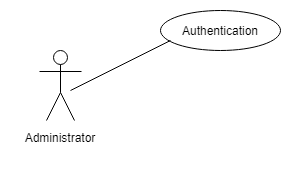
\includegraphics[scale=1]{diagrams/use.png}
\end{figure}
\begin{itemize}
\item Administrator: A default administrator account will be on the database and the administrator need to only login to access the administrator interface. The administrator of the system will receive a guideline pdf on the details of the administrator password and username and how to change the details if required.
\end{itemize}

\subsection{Domain Model}
\begin{figure}[h]
\centering
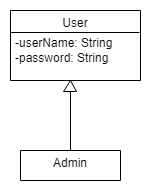
\includegraphics[scale=1]{diagrams/usedom.png}
\end{figure}
\subsection{Service Contracts}
The following services should be provided
Precondition: adminName is a registered user
Exception: If adminName is not a registered user throw \\noSuchAdmin exception
Postcondition: No change
\begin{figure}[h]
\centering
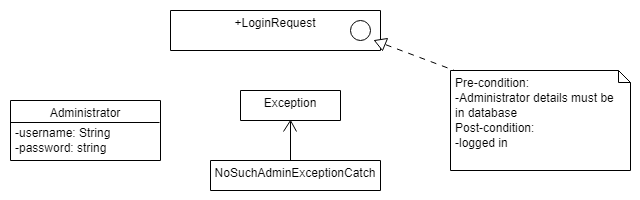
\includegraphics[scale=0.7]{diagrams/useS.png}
\end{figure}
\section{Catalogue Management Module}
\subsection{Scope}
The catalogue management module will allow the administrator to add, remove and update any items in the catalogue list.
The catalogue management module will also allow the  administrator to add specials to the module. Specials can be applied to singular items or groups of items depending on a special group configuration.
\begin{figure}[h]
\centering
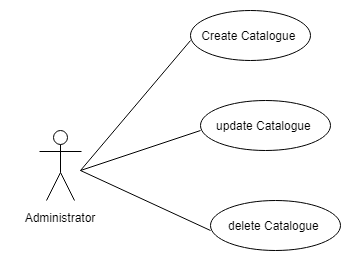
\includegraphics[scale=0.575]{diagrams/notS.png}
\end{figure}
\newpage
\subsection{Domain Model}
The domain model for the Catalogue Managemen system is simple. It is simply a description how the  catalogues can be modified by either being created, being updated or being deleted.
\begin{figure}[h]
\centering
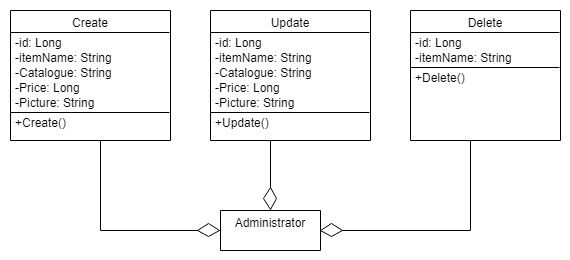
\includegraphics[scale=0.7]{diagrams/notdom.png}
\end{figure}
\newpage
\subsection{Service Contracts}
\begin{figure}[h]
\centering
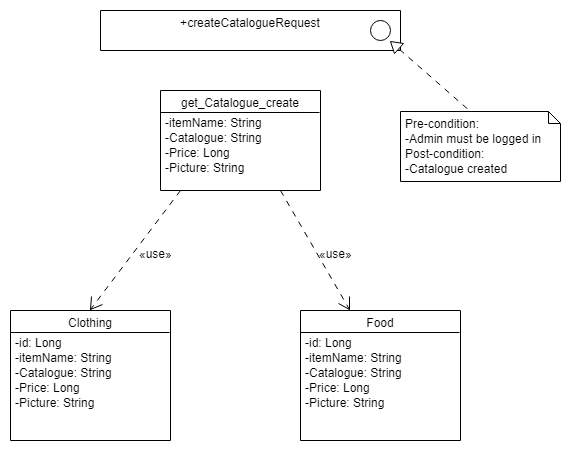
\includegraphics[scale=0.4]{diagrams/notC.png}
\end{figure}
\begin{figure}[h]
\centering
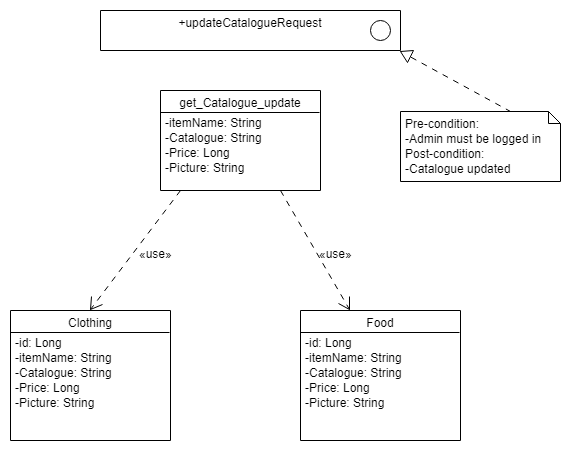
\includegraphics[scale=0.4]{diagrams/notSeq.png}
\end{figure}
\begin{figure}[h]
\centering
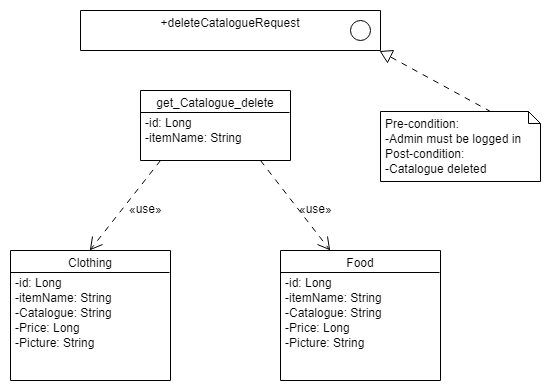
\includegraphics[scale=0.5]{diagrams/notSeqD.png}
\end{figure}

\newpage
\section{View Module}
\subsection{Scope}
The view module will allow the guest user to browse, search and alter the catalogues.

\begin{figure}[h]
\centering
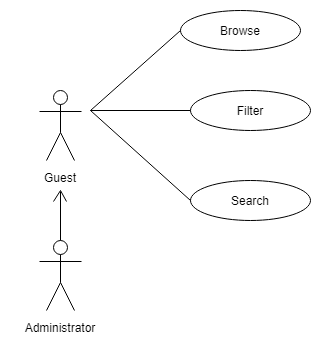
\includegraphics[scale=0.5]{diagrams/dataS.png}
\end{figure}
\newpage
\subsection{Domain Model}
\begin{figure}[h]
\centering
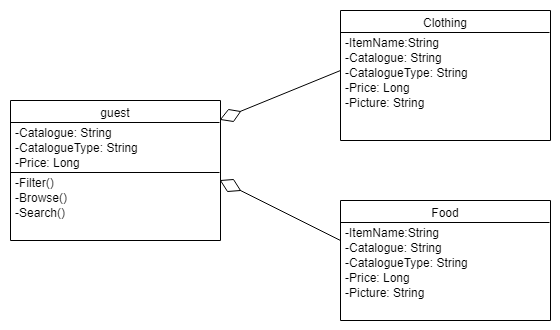
\includegraphics[scale=0.7]{diagrams/dataDom.png}
\end{figure}.
\newpage

\subsection{Service Contracts}
\begin{figure}[h]
\centering
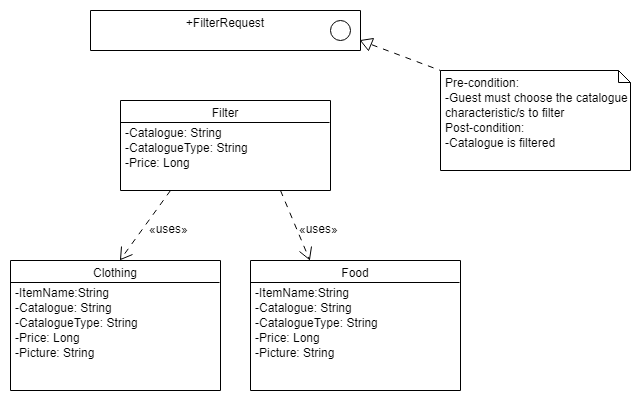
\includegraphics[scale=0.4]{diagrams/servView.png}
\end{figure}
\begin{figure}[h]
\centering
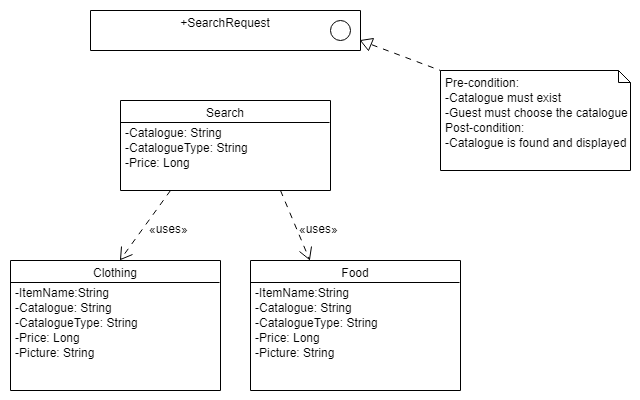
\includegraphics[scale=0.4]{diagrams/searchView.png}
\end{figure}

\section{Architectural Technologies}
The web application will consist of two subsystems that communicate via HTTP using REST Framework. The
Java/Spring Boot application will be known as the "backend" application. The HTML5/Angular2 application
will be known as the "frontend" application. The backend application is expected to communicate with the
database and use Hibernate which can be imported into Maven, a dependency management tool whereas the
frontend application will be hosted in the browser and NodeJS is expected to manage packages required for the
application to run successfully.

\subsection{Technologies}
The following technologies will be used to implement the system:
\begin{itemize}
\item Html 5 (Html and Bootstrap CSS)
\item Angular2
\item NodeJS
\item Spring Boot
\item PostgresSQL
\item Apache Maven
\item Git (Github)
\end{itemize}

\subsection{Monolithic Implementation}
The monolithic implementation will consist of one backend spring boot\\ application that will be deployed as a
single unit. Apache Maven will be used as the dependency management tool.


\end{document}